\documentclass[a5paper]{tufte-book}

\usepackage[caption=false]{subfig}
\usepackage{url}
\usepackage{graphicx}
\usepackage{listings}

\lstset{language=C}

% This document is intended to be read by 8 to 10 year old students.  Edits to
% the language should keep this in mind.

\title{Mobile Temperature Reader}
\author{}
\date{}

\begin{document}
\maketitle

\section*{Go, go, technology!}
We're going to make a thermometer.  But not just any thermometer!  Ours will be a super special Internet connected thermometer.  We'll make our own little computer and a circuit to read the temperature.  The temperature will be sent to our server on the Internet\marginnote{\url{http://wildfly8-ontoed.rhcloud.com/Temperature/}}.  Then anyone who wants to read the current temperature can read it.

The first task is to make the circuit, which you can see in figure~\ref{fig:circuit}.

\begin{figure}
  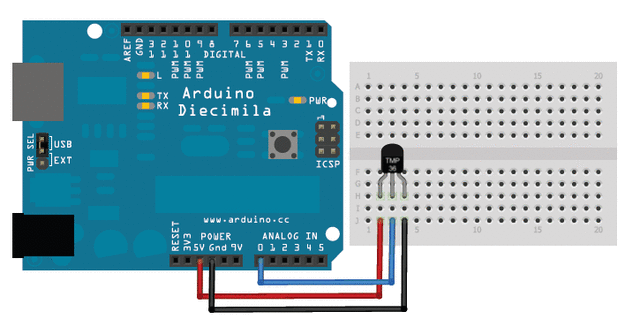
\includegraphics[width=\textwidth]{images/temperature_tmp36fritz}
  \caption{A circuit from \url{https://learn.adafruit.com/assets/476}}
  \label{fig:circuit}
\end{figure}

\section*{Fused}

Now we need to read a temperature from using the temperature sensor in this circuit.\marginnote{Code is modified from\url{http://playground.arduino.cc/Main/LM35HigherResolution}}

\begin{lstlisting}
float tempC;
int reading;
int tempPin = 0;

void setup() {
  Serial.begin(9600);
  analogReference(INTERNAL);
}

void loop() {
  reading = analogRead(tempPin);
  tempC = reading / 9.31;
  Serial.println(tempC);
  delay(2000); // wait 2 seconds
}

\end{lstlisting}

\section*{Super Fused}
Finally, and this is the big job, we need to send this data up to our server.  There's a lot of work in telling such a simple device to send information through the Internet.  A code listing that achieves this can be seen in the following listing.\marginnote{This code is mostly from \url{http://playground.arduino.cc/Code/WebClient}}

\begin{lstlisting}
  #include <SPI.h>
  #include <Ethernet.h>

  byte mac[] = {0xDE, 0xAD, 0xBE, 0xEF, 0xFE, 0xED};

  // initialize the library instance:
  EthernetClient client;

  char server[] = "wildfly8-ontoed.rhcloud.com";

  unsigned long lastConnectionTime = 0;
  boolean lastConnected = false;
  const unsigned long postingInterval = 60L*1000L;

  void setup() {
    // start serial port:
    Serial.begin(9600);
    // give the ethernet module time to boot up:
    delay(1000);
    // start the Ethernet connection and get an IP address via DHCP
    Ethernet.begin(mac);
  }

  void loop() {
    // if there's incoming data from the net connection.
    // send it out the serial port.
    if (client.available()) {
      char c = client.read();
      Serial.print(c);
    }

    // if there's no net connection, but there was one last time
    // through the loop, then stop the client:
    if (!client.connected() && lastConnected) {
      Serial.println();
      Serial.println("disconnecting.");
      client.stop();
    }

    // if you're not connected, and ten seconds have passed since
    // your last connection, then connect again and send data:
    if(!client.connected() && (millis() - lastConnectionTime > postingInterval)) {
      httpRequest(98.0f);
    }
    // store the state of the connection for next time through
    // the loop:
    lastConnected = client.connected();
  }

  // this method makes a HTTP connection to the server:
  void httpRequest(float temperature) {
    // if there's a successful connection:
    if (client.connect(server, 80)) {
      char postRequest[64];
      sprintf(postRequest, "POST /Temperature/%f HTTP/1.1", temperature);
      Serial.println("connecting...");
      // send the HTTP POST request:
      client.println(postRequest);
      client.println("Host: wildfly8-ontoed.rhcloud.com");
      client.println("Accept: application/json");
      client.println("Connection: close");
      client.println();

      // note the time that the connection was made:
      lastConnectionTime = millis();
    } else {
      // if you couldn't make a connection:
      Serial.println("connection failed");
      Serial.println("disconnecting.");
      client.stop();
    }
  }
\end{lstlisting}

\end{document}